\subsection{Stakeholder}
\label{sec:Kap-6.1.1}

Es ist durchaus nicht trivial, mit einem Softwareprodukt die Bedürfnisse der zukünftigen Nutzer zu treffen. Denn in der Regel wird es nicht nur für eine Nutzergruppe, sondern für eine Menge sehr heterogener Teilgruppen mit eventuell widerstreitenden Bedürfnissen entwickelt. Zum Beispiel könnten bei den zukünftigen Nutzern unterschiedliche fachliche Hintergründe bzw. Arbeitsschwerpunkte vorliegen (wie \zb im Zookontext Tierpfleger, Mitarbeiter an der Zookasse, Verwaltungsmitarbeiter, IT-Personal) oder die Gruppen könnten unterschiedlich viel Erfahrung im Umgang mit Software haben. Ein anderer Unterschied könnte darin bestehen, wie lange oder wie intensiv jemand das Softwareprodukt täglich einsetzen muss. 

Um von konkreten Personen (\zb Tierpfleger Helmut, der sehr IT-erfahren ist und das Softwareprodukt ca. eine halbe Stunde pro Tag nutzen wird) zu abstrahieren, verwendet man auch im Requirements Engineering den Begriff der Rolle, \marginline{Rolle}
den wir schon im Kontext der Zusammensetzung des Entwicklungsteams in Abschnitt 1.2.2 % TODO Abschnitt~\ref{sec:Kap-1.3.2}
vorgestellt hatten. Im Rahmen des Requirements Engineering geht es allerdings nicht um Rollen während der \textbf{Entwicklung} des Softwareprodukts, sondern um eingenommene Rollen bei dessen \textbf{Nutzung}. Unterschiedliche Rollen stellen unterschiedliche Anforderungen an das Softwareprodukt, zum Beispiel weil sie verschiedene Funktionalitäten nutzen werden (\zb Rolle Tierpfleger vs. Rolle Mitarbeiter der Zoo\-verwaltung) oder die Software für sie unterschiedlich stark intuitiv zu nutzen sein muss (\zb Rolle IT-erfahrener Nutzer vs. Rolle IT-unerfahrener Nutzer).

Die verschiedenen (zukünftigen) Nutzerrollen sind jedoch bei Weitem nicht die einzigen Stakeholder, die Anforderungen an das Softwareprodukt stellen werden. Zu den im Requirements Engineering relevanten Stakeholdern gehören eine Reihe weiterer Personengruppen, darunter auch solche, die das Softwareprodukt später gar nicht selber nutzen werden. Mögliche Stakeholder eines Softwareentwicklungsprozesses im Rahmen des Requirements Engineering sind:

\begin{itemize}
	\setlength{\itemsep}{0.4mm} %%% für Druck
	
	\item \textbf{Nutzer des Softwareprodukts}: wie beschrieben, handelt es sich häufig um eine sehr heterogene Gruppe mit unterschiedlichen, teilweise auch wider\-streitenden Interessen. Die Anforderungen der Nutzer beziehen sich in der Regel auf das Vorhandensein gewünschter Funktionalitäten und auf Aspekte wie die einfache Bedienbarkeit der Software.
	\item \textbf{Führungsebene des Auftraggebers}: diejenigen Personen(gruppen), die entscheiden, dass das Softwareentwicklungsprojekt durchgeführt wird und Ressourcen für das Projekt bewilligen. Wenn es sich nicht um eine Auftragsarbeit, sondern um eine Entwicklung für die eigene Institution bzw. eine Entwicklung zum Verkauf auf dem kommerziellen Markt handelt, handelt es sich bei diesem Stakeholder um die Führungsebene des eigenen Hauses. Dieser Stakeholder definiert, welche (Unternehmens)Ziele durch das zu entwickelnde Softwareprodukt erreicht werden sollen und er entscheidet zum Beispiel auch, welche Mitarbeiter als Domänenexperten für das Projekt abgestellt werden (können). Neben Anforderungen an den Entwicklungsprozess, wie die Einhaltung von Kosten- und Zeitplänen, könnte er auch konkrete Anforderungen an das Softwareprodukt stellen, zum Beispiel, dass dieses umfangreiche Hilfestellungen zu den einzelnen Funktionalitäten beinhalten muss, damit der spätere Schulungsaufwand für seine Mitarbeiter gering bleibt, oder dass es mit der bestehenden Hardware kompatibel sein muss, damit nicht neue Hardware für die Mitarbeiter gekauft werden muss.
	\item \textbf{IT-Abteilung des Auftraggebers}: Diesem Stakeholder könnte wichtig sein, dass das neue Produkt gut in die Haus-IT eingepasst werden kann, zum Beispiel indem es entsprechende Schnittstellen zu anderen verwendeten Softwareprodukten im Haus hat. Des Weiteren werden aus dieser Richtung Anforderungen im Hinblick auf Betrieb und Wartung des zukünftigen Softwareprodukts kommen.
	\item \textbf{Verwaltung des Auftraggebers}: Der Einsatz des neuen Produkts kann auch Auswirkungen auf Bereiche außerhalb der Fachabteilungen, für die es gedacht ist, haben. Wenn zum Beispiel im Zookontext die Futterbeschaffung für die
	\linebreak %%% für Druck
	Tiere bisher von den einzelnen Tierpflegern übernommen wurde und jetzt mit der neuen Software zentral organisiert werden soll, ändern sich Arbeits\-prozesse im Einkauf. Die dortigen Mitarbeiter werden entsprechend Anforderungen (\zb die Speicherung verwaltungsrelevanter Informationen) an das Softwareprodukt stellen.
	\item \textbf{Marketing/ Öffentlichkeitsarbeit/ Pressestelle etc. des 
	Auftrag- \linebreak
	gebers}: Dieser Stakeholder wird nach Möglichkeiten suchen, wie das neue Produkt in die Öffentlichkeitsarbeit des Unternehmens eingebunden werden kann bzw. diese vereinfachen kann. Wenn ein Produkt für den kommerziellen Markt entwickelt wird, nimmt dieser Stakeholder eine besonders zentrale Rolle ein, aber auch bei der (individualisierten) Entwicklung für einen Auftraggeber oder für das eigene Haus können Anforderungen aus dieser Richtung kommen. Zum Beispiel könnte die Pressestelle des Zoos die Anforderung stellen, dass das Softwareprodukt automatisiert bei jeder Geburt im Zoo eine entsprechende Pressemitteilung an die regionalen Zeitungen versendet.
	\item \textbf{Mitarbeiter der Qualitätssicherung des Auftraggebers}: Von diesem Stakeholder sind Anforderungen bezüglich der Einhaltung von (unternehmenseinheitlichen) Prozessen und Standards, aber -- bezogen auf das Software\-produkt -- auch Anforderungen zur Bedienbarkeit der Software und zum Vorhandensein spezifischer Testfälle, die Qualitätskriterien der Software über\-prüfen, zu erwarten.
	\item \textbf{Betriebsrat des Auftraggebers}: Dieser Stakeholder könnte zum Beispiel Anforderungen bzw. Bedingungen formulieren, welche Informationen die Software erheben darf, wenn Mitarbeiter sie nutzen. Zudem werden durch die mögliche Änderung von Arbeitsprozessen durch das Softwareprodukt die \mbox{Interessen} dieses Stakeholders berührt.
	\item \textbf{Kunden des Auftraggebers}: wie zum Beispiel im Zookontext die Besucher des Zoos. Auch die Bedürfnisse dieser Gruppe sollten nicht unberücksichtigt bleiben, denn sie werden häufig der Grund sein, weshalb der Auftraggeber überhaupt ein Softwareprodukt entwickeln bzw. verbessern lassen möchte. In der Regel werden die Kunden des Auftraggebers nicht direkt an der Anforderungsermittlung mitwirken, sondern der Auftraggeber muss ihre Bedürfnisse mitdenken (vielleicht sogar durch Befragungen oder Ähnliches im Vorfeld erhoben haben) und -- sofern sie zu seinen Zielen passen -- als Anforderungen an das Softwareprodukt formulieren.
	\item \textbf{Betriebliche oder staatliche Datenschutzbeauftragte}: Aus dieser Richtung sind vor allem Anforderungen zu den von der Software verarbeiteten Daten zu erwarten. In Bereichen, in denen besonders schützenswerte personenbezogene Daten verarbeitet werden (\zb Software im Gesundheitsumfeld) hat dieser Stakeholder eine besonders zentrale Rolle. Aber auch das im Zoobeispiel von der Zoodirektorin vorgesehene Veröffentlichen der Namen der Tierpfleger berührt schon die Interessen dieses Stakeholders.
	\item \textbf{Aufsichtsbehörden/ Prüfer/ Sicherheitsexperten}: Je nach Domäne und Einsatzzweck des Softwareprodukts müssen unterschiedlich strenge gesetzliche Vorschriften eingehalten werden. Entsprechende Anforderungen von diesem Stakeholder werden nicht nur von konkreten Personen gestellt, sondern finden sich auch in Gesetzen und Richtlinien, die das Softwareentwicklungsprojekt berücksichtigen muss.
	\item \textbf{Schulungs- und Servicepersonal des Auftraggebers oder Auftrag\-nehmers}: Diese Personen haben die Aufgabe, die Nutzer in der Verwendung des Softwareprodukts zu schulen und ihnen bei Problemen zu helfen. Unabhängig davon, ob dieser Stakeholder beim Auftraggeber angesiedelt ist oder bei dem Unternehmen, das das Softwareprodukt erstellt hat, wird er Anforderungen in Bezug auf die einfache Bedienbarkeit der Software und auf das Vorhandensein von Dokumentationen zur Software stellen.
	\item \textbf{Auftragnehmer}: Auch das Unternehmen, das das Softwareprodukt erstellt, bzw. bei Eigenentwicklung die entsprechende Abteilung, kann ein 
	Stake- \linebreak %%% für Druck
	holder im Softwareentwicklungsprozess sein. Das kann Beschränkungen bezüglich möglicher Programmiersprachen oder Entwicklungstechniken für das Software\-produkt betreffen, zum Beispiel kann evtl. nicht in C$++$ implementiert werden, wenn das Personal nur aus Java-Entwicklern besteht. Es könnte von diesem Stakeholder aber auch gewünscht sein, zu entwickelnde Komponenten möglichst wiederverwendbar zu gestalten, um sie auch in anderen Softwareentwicklungsprojekten einsetzen zu können. Letztere Anforderung wird häufig nicht explizit formuliert werden, insbesondere wenn für einen externen Auftraggeber entwickelt wird oder eine solche Anforderung an eine Komponente mit Anforderungen anderer Stakeholder kollidieren würde.
\end{itemize}

Es ist sehr projektspezifisch, welche Gruppen genau zu den Stakeholdern gehören. Neben den Zielen und dem Produktumfang der zukünftigen Software ist dies auch abhängig von der Domäne sowie der Struktur und Größe des Unternehmens des Auftraggebers (\zb hat nicht jedes Unternehmen einen Qualitätssicherungsexperten und vielleicht auch keine eigene IT-Abteilung). Zudem werden nicht alle Stakeholder für das Gelingen des Projekts gleich wichtig sein. In jedem Fall gibt es für ein Softwareentwicklungsprojekt aber oft deutlich mehr zu berücksichtigende Stakeholder als man im ersten Moment denken würde.

Da alle diese Stakeholder potentielle Lieferanten von Anforderungen sind, ist es für das Softwareentwicklungsteam bzw. dessen Projektleiter wichtig, diese möglichst zu Beginn des Projekts zu kennen bzw. in Erfahrung zu bringen. Wenn Stakeholder unberücksichtigt bleiben, bleiben -- nicht immer, aber häufig -- auch deren Anforderungen unberücksichtigt. Und nach Murphys Gesetz (anything that \textbf{can} go wrong \textbf{will} go wrong) werden diese unberücksichtigten Anforderungen im späteren Projekt\-verlauf oder nach Einführung des Softwareprodukts doch prioritär werden und (unter Umständen umfangreiche und kostenintensive) Änderungen an der Software erforderlich machen. Insofern müssen (und werden) bei der Anforderungsermittlung nicht alle Stakeholder persönlich anwesend sein, aber ihre Interessen sollten immer mit am Tisch sitzen. In der Praxis gibt es häufig von Seiten des Auftraggebers intern vor Projektstart abgestimmte Aufstellungen von Anforderungen, die schon die Interessen mehrerer Stakeholder vereinen und zumindest eine erste Basis für die Anforderungsermittlung bilden.

\vspace{1.5mm} %%% für Druck

Die \marginline{Konflikt\-potenzial} Berücksichtigung und Priorisierung der Anforderungen verschiedener Stake\-holder kann enormes Konfliktpotenzial bieten, insbesondere dann, wenn mit den vorgesehenen Ressourcen nicht alle Anforderungen umgesetzt werden können oder sich Anforderungen verschiedener Stakeholder nicht miteinander vereinbaren lassen. Hinzu kommt, dass Stakeholder neben den Interessen, die sich aus ihrer Position oder ihren Arbeitsschwerpunkten ergeben, auch persönliche Interessen haben, die mit\-unter ihren Weg in die Anforderungen finden. Zum Beispiel könnten sich Mitarbeiter wünschen, dass das zukünftige Softwareprodukt sie von lästigen Routineaufgaben befreit und entsprechende Anforderungen höher priorisieren als es den eigentlichen Zielen des Softwareentwicklungsprojekts entspricht. Auf der anderen Seite könnten zukünftige Nutzer versuchen, alle Funktionalitäten zu verhindern, die ihre bisherigen Arbeitsprozesse verändern. Aus Sicht des Entwicklungsteams des Softwareprodukts ist es zentral, dass es ganz klare Regeln gibt, welche Mitarbeiter des Auftraggebers direkt Anforderungen stellen oder priorisieren dürfen und welche ihre Interessen dem Entwicklungsteam nur indirekt über festgelegte Ansprechpartner des Auftraggebers mitteilen können. Diese Entscheidung trifft die Führungsebene des Auftraggebers bzw. ein von ihr benannter Entscheidungsträger. Meistens ist es allerdings keine gute Option, allen anderen Personen des Unternehmens den Zugang zum Entwicklungsteam zu verweigern, da letzterem damit auch Quellen für Domänenwissen vorenthalten werden könnten. Zumal es in der Praxis auch nicht selten vorkommt, dass der benannte Ansprechpartner für das Entwicklungsteam die Domäne deutlich weniger gut kennt als andere Mitarbeiter des Unternehmens.

\vspace{\baselineskip} %%% für Druck

\minisec{Stakeholderpflege in agilen Projekten}

Die frühe Kenntnis der potenziellen Stakeholder ist auch in agilen Softwareentwicklungsprojekten sehr wichtig, auch wenn diese die Möglichkeit von Anforderungs\-änderungen über die komplette Projektlaufzeit vorsehen. Die Schwierigkeit liegt hier weniger darin, dass \textbf{überhaupt} neue Anforderungen gestellt werden. Diese können (mit mehr oder weniger Anpassungen am bestehenden Programmcode) in späteren Iterationen umgesetzt werden. Problematisch kann es aber werden, wenn neue Stake\-holder die schon bearbeiteten Anforderungen oder die Art und Weise wie diese umgesetzt wurden, \textbf{grundsätzlich} in Frage stellen. 

\vspace{1.5mm} %%% für Druck

Das agile Vorgehensmodell Scrum geht einen sehr rigorosen Weg, um die möglichen Zielkonflikte zwischen Stakeholdern vom Entwicklungsteam fernzuhalten. Die \marginline{die Rolle Product Owner} Rolle des Product Owner, der die Anforderungen priorisiert, wird nur von genau einer (vom Auftraggeber zu benennenden) Person übernommen. Von der fachlichen Seite bestimmt nur der Product Owner, welche Anforderungen in der nächsten Iteration umgesetzt werden sollen. In der Praxis wird der Product Owner zwar weitere Mit\-arbeiter des Auftraggebers einbinden (müssen), indem er diese Anforderungen formulieren lässt oder sie sogar als Domänenexperten direkt mit ins Projekt einbezieht. Entscheider aus Sicht des Entwicklungsteams bleibt aber ausschließlich der Product Owner, unabhängig davon wie viele andere Personen an Besprechungen teilnehmen, Ideen oder Anforderungen äußern. Die Rolle Product Owner ist kein einfacher Job. Sie muss jederzeit den Überblick über das Gesamtprodukt haben und wissen, welche Anforderungen die höchste Priorität erhalten sollen, die Fragen der Entwickler zur Domäne und zu den Anforderungen beantworten können bzw. Personen benennen können, die dazu in der Lage sind, dabei die Interessen aller Stakeholder berücksichtigen und deren Konflikte lösen und gleichzeitig ihrer Führungsebene regelmäßig über den Stand des Projekts berichten.

\vspace{\baselineskip} %%% für Druck

\minisec{Identifizieren und Dokumentieren der Stakeholder}

Es gibt in der Literatur zahlreiche praktische Hinweise und Methoden, wie sich die Stakeholder für ein Softwareentwicklungsprojekt bestimmen lassen, wie man ihre Interessen und Ziele dokumentieren kann und wie sich die Wichtigkeit einzelner Stakeholder bewerten lässt.

\begin{figure}[h!]
	\centering
	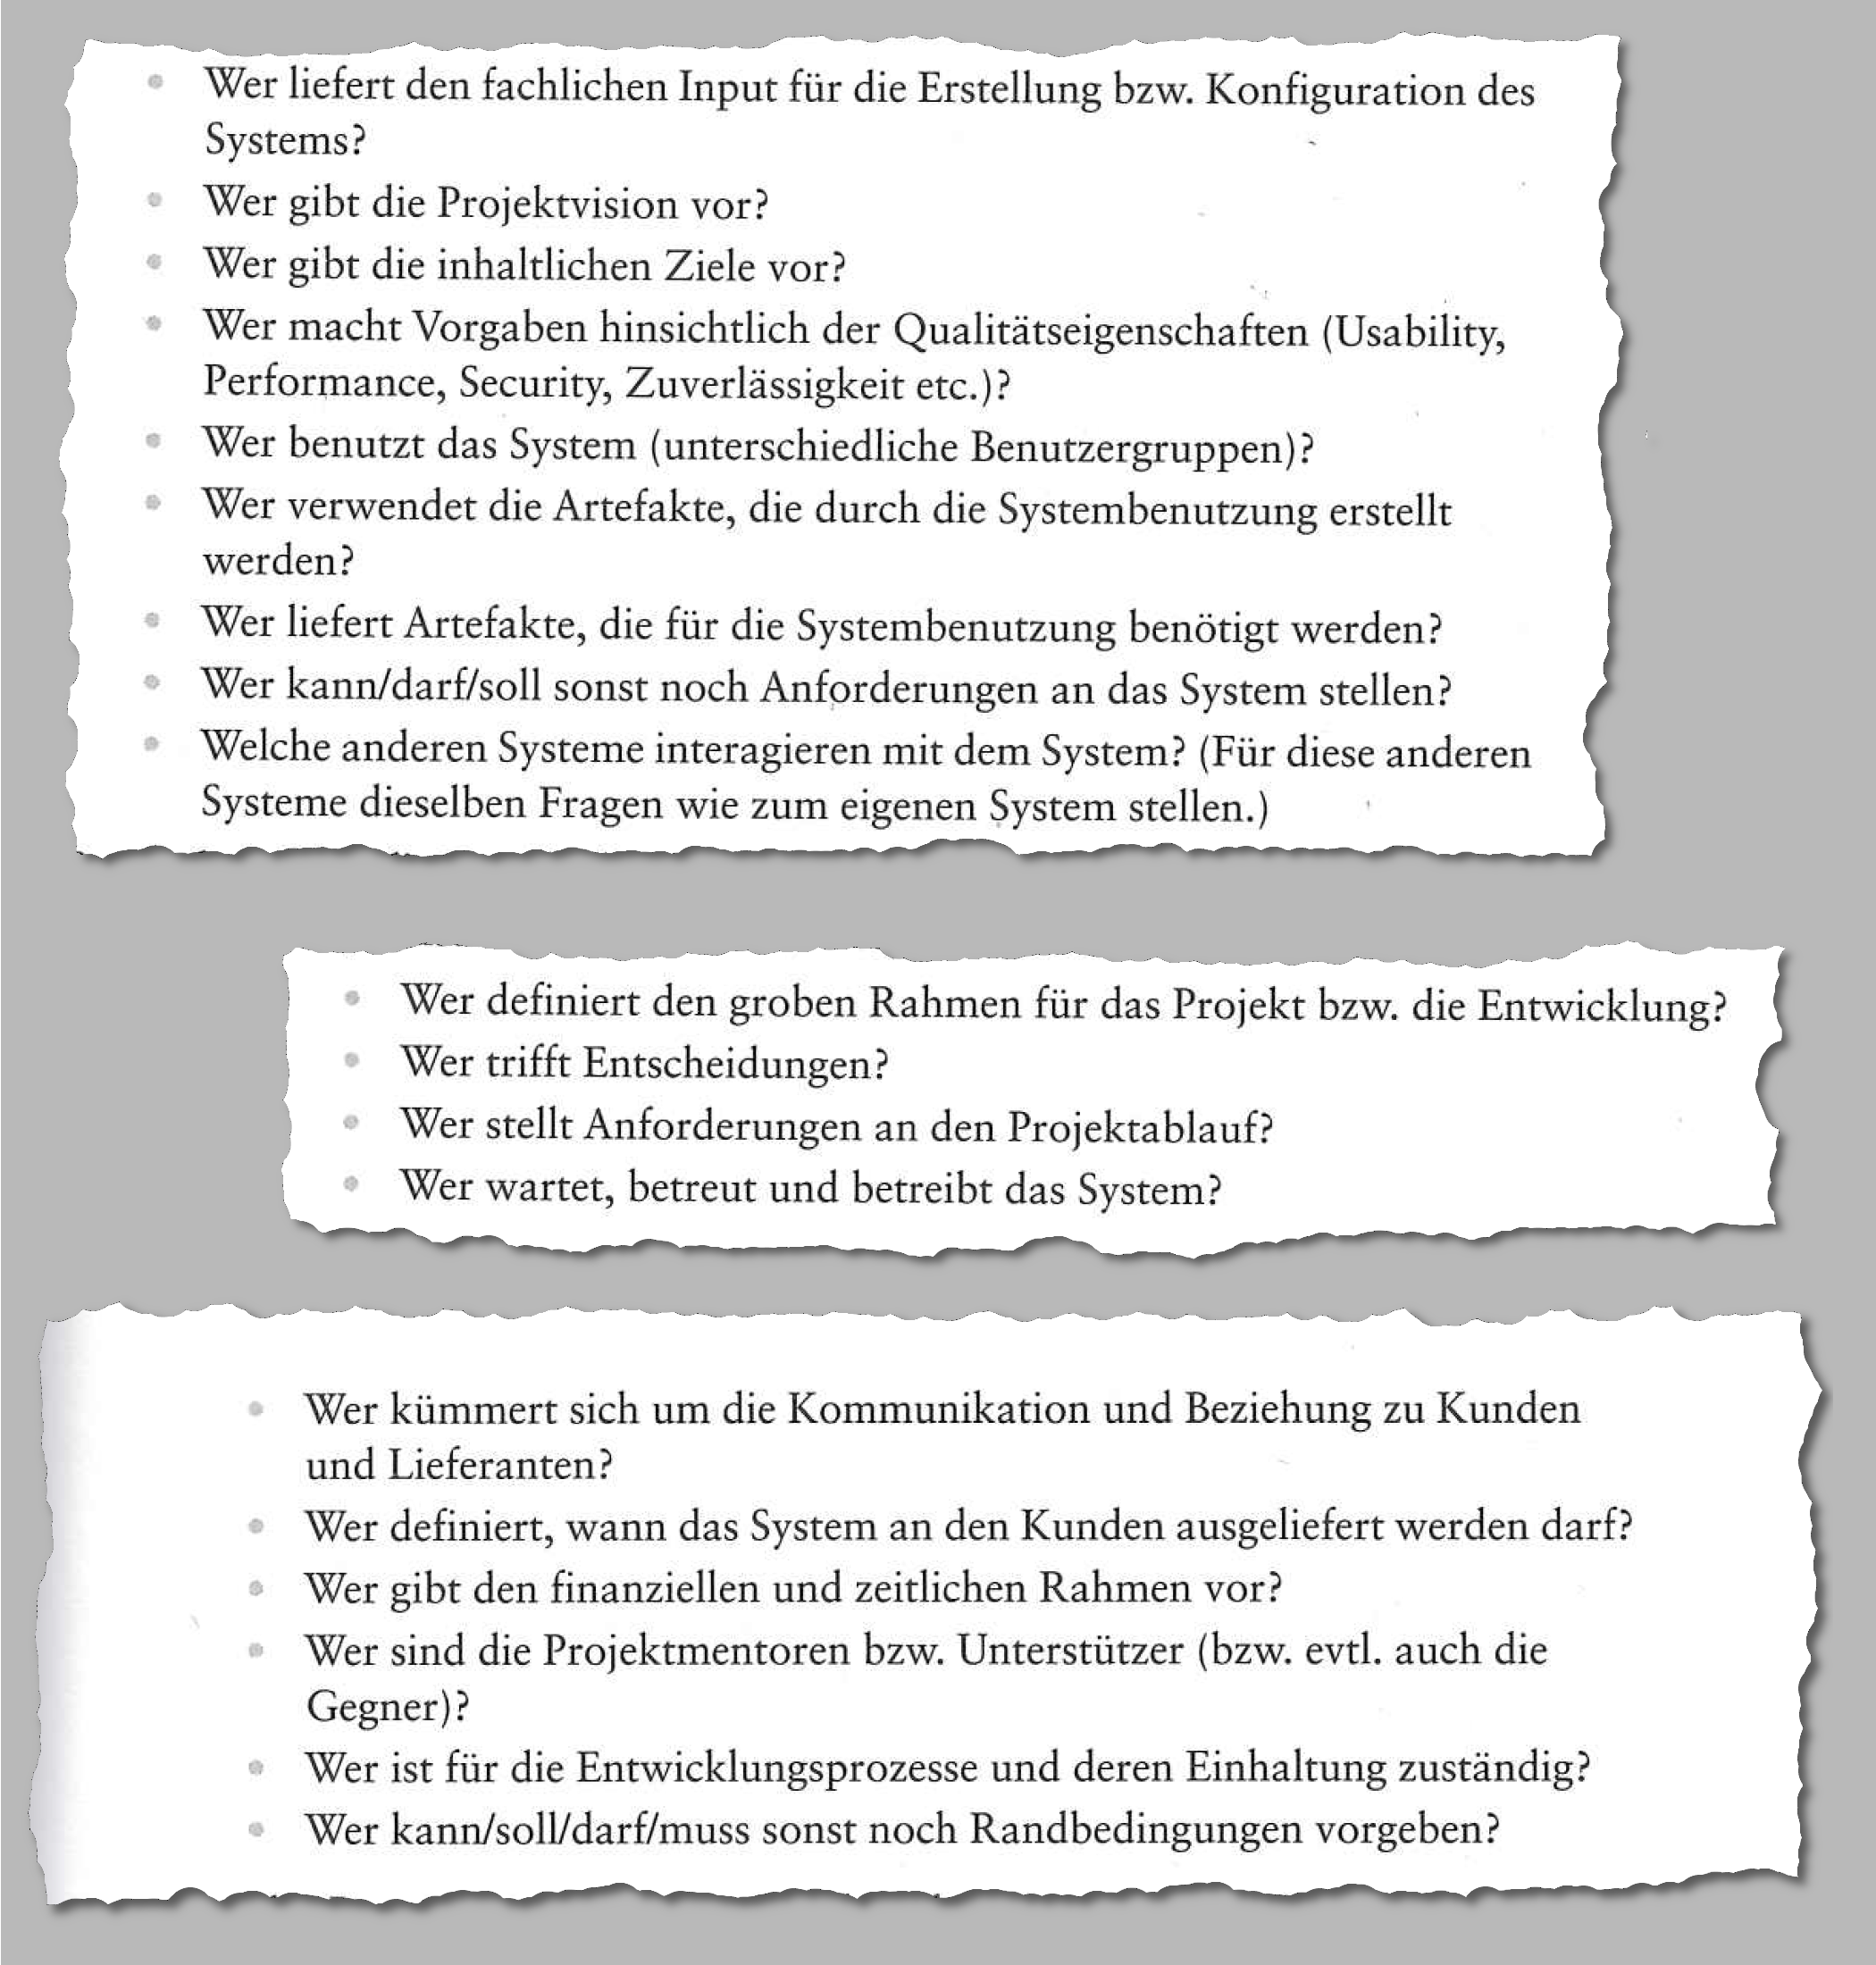
\includegraphics[width=\textwidth]{Bilder/Kapitel-6/Stakeholder_Medley_V2.png}
	\caption[Mögliche Fragen zur Identifizierung von Stakeholdern]{Mögliche Fragen zur Identifizierung von Stakeholdern. Inhalte aus: \cite[84 \psq]{ber18}}
	\label{fig:stakeholder_medley}
	
	\vspace{\baselineskip} %%% für Druck
\end{figure}

Eine Möglichkeit, Stakeholder zu bestimmen, ist dem vom Auftraggeber genannten Ansprechpartner schematische Fragen der Art, „Wer wartet und betreut das zukünftige System?“, „Wer definiert die inhaltlichen Ziele?“, „Wer bestimmt üblicherweise den Projektablauf durchzuführender Projekte?“ zu stellen und auf diese Weise \mbox{Namen} von weiteren Mitarbeitern oder Hinweise auf Organisationseinheiten des Unternehmens zu erhalten, die potenzielle Stakeholder sein könnten. Abbildung~\ref{fig:stakeholder_medley} zeigt Ausschnitte aus Fragenlisten von \cite[84 \psq]{ber18}. Weitere Listen solcher Fragen, an denen man sich orientieren kann, finden Sie bei \cite[36]{lap17} und \cite[122 \psqq]{lef11}.

Bei \cite[55 \psqq]{ebe22} finden 
\marginline{weiterführende Literatur}
Sie eine praktische Stakeholder-Analyse in acht Schritten, mit der Stakeholder, ihre Interessen und Konfliktpotenziale zwischen Stake\-holdern identifiziert und dokumentiert werden können. \cite[44 \psq]{rob13} stellt mit der sogenannten Stakeholder Map zudem eine Möglichkeit vor, Stakeholder und ihre Beziehungen zueinander in größeren Einheiten zu kategorisieren und zu visualisieren. \cite[48 \psq]{oes13} stellt eine Methode zur Bewertung der Wichtigkeit eines Stakeholders vor, die das Risiko, diesen Stakeholder nicht zu  berücksichtigen und den benötigten Aufwand seine Interessen zu erkunden ins Verhältnis setzt. \cite[81 \psqq]{rup14} zeigt Beispiele für Schablonen zur Dokumentation von Stakeholdern, \mbox{ihren} Interessen und Einflussmöglichkeiten und stellt ein Stakeholder-Analysemodell vor, mit dem Stake\-holder anhand der Kriterien Einfluss und Motivation gruppiert werden können. \cite[121]{lef11} und \cite[46 \psq]{lap17} zeigen Beispiele für Stakeholder-
\linebreak %%% für Druck
Rankings. 
